\documentclass[a4paper]{acm_proc_article-sp}  
\usepackage{microtype}
\usepackage{mathpazo}
\usepackage{listings}
\usepackage{xspace}
\newcommand{\eg}{e.g.\@\xspace}
\newcommand{\ie}{i.e.\@\xspace}
\newcommand{\etc}{etc.\@\xspace}
\newcommand{\Naive}{Na\"{i}ve\@\xspace}
\newcommand{\naive}{na\"{i}ve\@\xspace}
\lstset{language=python}
\begin{document}

%%%Kubi+Anthony comments
%%%trigger on sensors
%%%us vs. other watering systems (ETO)
%%%weather.com XML weather
%%%we can provide the cloud
%%%more pics

\title{FRAICHE: Fast Response And Intelligently Controlled Harvest Environment}
\author{\alignauthor Peggy Chi, Jonathan Kummerfeld, Valkyrie Savage \\
\affaddr{Computer Science Division\\University of California, Berkeley} \\
\email{\{peggychi, jkk, valkyrie\}@cs.berkeley.edu}\\
\text{CS262A Final Project, Fall 2012}
} 
\maketitle

\setcounter{page}{1}
\pagenumbering{arabic}

\section{Abstract}

FRAICHE is a complete small-scale sensing and watering system for deployment in community gardens.  The goal is to provide gardeners with sophisticated monitoring and analysis of their garden at low cost in an easy to set up system.  We achieved this by constructing a central server that receives sensors readings, models the environment to makes predictions about future moisture content, and responds to user queries made through a straightforward web interface.  FRAICHE is implemented using a Raspberry Pi, a system with minimal computing power, which poses a challenge since our goal is to provide fresh predictions when queries are received, but with minimal latency.  We considered six methods of scheduling model updates, and tested them under three very different use-case scenarios, finding that in each case we can strike an effective balance between freshness and latency.

\section{Introduction}

Managing a community garden or small farm is currently a process that requires community members or the farmer to directly monitor their land in an ad-hoc manner.  Additionally, beginning gardeners who lack a large base of knowledge sometimes find it difficult to react effectively to the signals they see coming from their plants, watering them to the point of drowning or failing to notice when they are parched.  Computing has been leveraged to improve the ease of interaction with and analysis of many other physical processes, and is a natural addition here, where continuous monitoring and effective predictions of soil moisture content can provide crucial information.

FRAICHE is a system with both sensing and watering capabilities. It can deliver information to the owner about a range of factors, such as moisture and temperature status of the soil around different plants, via a web app. The same web app allows them to water plants or schedule their watering, with the actual watering accomplished through a configurable drip irrigation system. The system also provides predictions about future soil moisture content, based on a range of different factors. These predictions are tuned to the particular garden being used, with values predicted based on past observed changes.

We implemented a complete, small scale system to test computation bottleneck issues for our implementation, particularly for how the sensors being used will manage communication with the central controller. To stress test the system, we simulated a scaled up version. This version involves an extremely large number of sensors working in a star network, with a single central controller receiving data from sensors, updating models, and handling queries from users.  Constantly receiving sensor updates, using them to update the model, and maintaining low latency responses to clients is a reasonably simple problem with low overhead, but when running such a system on a machine like the Raspberry Pi that has little computational headroom, balancing these tasks becomes a challenge.

In light of this, we tried multiple options for improving response speed.  We implemented several different schedulers to balance the loads of serving clients, getting fresh sensor data, and updating the prediction model.  We also implemented a system whereby multiple Raspberry Pis functioning in separate gardens can load balance between themselves via a central data repository.

This work focuses on a particular use-case, gardening, but the question we are addressing is more general.  When using a low-computation device such as a Raspberry Pi what is the best way to schedule expensive computation?  Recent growth in the hobbyist community has seen an enormous range of applications for the device, which often include some form of sensing and a means of communication with users.  The issue of latency that we focus on here could be particularly important for cases such as cooking applications and games that include real-world objects.

Our experiments show that while all scheduling approaches are effective in small scale situations, as either the number of sensors or the number of users increases the decision of when to make model updates becomes much more important.  Our observations follow expectations, with low latency being easily achievable at the cost of freshness or vice versa, but with more balanced combinations being dependent on the use case.  Finally, we show that by taking traffic patterns into consideration we are able to provide fresh information with low latency.

\section{Related Work}

While the focus of this work is very specific, it is worth taking a broader view when considering related work.  The general problem of resource management is well-studied, as is load-balancing, which we consider when demonstrating an implementation with multiple Raspberry Pi boards.  For our more specific case of plant monitoring there has been work on various forms of environmental sensing, particularly recently with wireless mesh networks, but we only mention a few specific cases, as generally that work focuses on data collection followed by offline analysis, unlike our setup.

\subsection{Resource Management}
%TODO: Fill in cites, also make an editing pass
There has been a bevy of work on resource management for both parallel clusters and multiple virtual machines running on a single physical machine.

The Dominant Resource Fairness algorithm is designed to help allocate resources fairly in multi-resource systems where processes have heterogeneous demand [Ghodsi et al. 2011]. It is a port of max-min allocation where instead of considering a process's overall needs they are measured as vectors with entries per resource.  However, DRF is designed to work in a system where there are sufficient resources to satisfy all processes' needs, which is different from our situation on the Raspberry Pi.

Jockey is another resource management system, and it is built to hold processes to particular Service Level Objectives (SLOs) [Ferguson et al. 2012].  Jockey uses predictive algorithms to simulate each job and estimate the time to completion. FRAICHE differs in that we are aiming to serve models that are as fresh as possible to clients, and the access times of clients are not as well - or strictly defined as SLOs.

Lottery scheduling has been put to use for managing resources: the basic idea is to allot a certain number of tickets to each process requiring a resource based on that process's importance and relative need for the resource [Waldspurger and Weihl 1994]. FRAICHE's goals are not to schedule many processes fairly to run in minimal time, but rather to run the model refinement algorithms as close as possible to clients' requests for plant data.

For virtual machines sharing a physical computer, Xen has explored the resource management question [Barham et al. 2003].  However their main challenges lay in isolation of the various virtual machines from each other in order to ensure security, while our challenges lay mainly in scheduling.

Work on scheduling for parallel clusters has included Lithe [Pan et al. 2010], use of loosely-synchronized clocks, and others.  The goal for scheduling with parallel clusters, however, is based mainly on ordering of events when processes don't share a clock.  In contrast, FRAICHE focuses on just one machine on which events take place.

\subsection{P2P Network and Load Balancing}

Sharing available workstations in a distributed computing environment has been widely studied in the systems community. Nichols discussed a mechanism to run network server programs on idle workstations considering process invocation and machine registry [Nichols 1987]. Condor is a scheduling system that aims to utilize the performance by assigning background jobs to those idle workstations it "hunted" [Litzknow et al. 1988]. More recent systems including Pastry [Rowstron and Druschel 2001] and Chord [Stoica et al. 2001] design routing mechanisms to limit hops for a query in a peer-to-peer (P2P) framework. The multiple Pis scenario of FRAICHE consider these system designs to leverage the workload of one web server to other idle machines.

Our work is closely related to load balancing and load sharing designs in distributed networks. Harchol-Balter and Downey proposed a preemptive migration scheme for CPU load balancing using a trace-driven simulation [1997]. It required no a priori knowledge about the process behaviors in networks of workstations, which matches our scenario where community clients can freely access the plant data. Harish and Owens [1999] designed load balancing models and algorithms for DNS servers, which is a simple but effective mechanism.

\subsection{Environmental Monitoring}

There are several monitoring systems that share the similar purposes as ours. Macroscope is a wireless sensor network deployed in a 70-meter tall redwood tree [Tolle et al. 2005]. The measured data included air temperature, relative humidity, and solar radiation. Their case study in practice addressed challenges of extracting meaningful information from the collected data and physical installation. 

Other sensor network systems targeted on different scenarios: Cardell-Oliver et al. designed an event-driven network to monitor soil moisture to measure water flow [2004]. Their environment reactive design consider the rainfall conditions: only when rain falls that causes rapid soil moisture changes, the measurements are collected frequently. PipeProbe is a mobile sensor system that constructs spatial topology of water pipelines by reading sensor capsule data [Lai et al. 2010]. These projects demonstrated the practical designs deployed in the real world, and therefore inspired us to monitor and provide prediction by modeling the moisture data.

%%%\section{Background}

\section{Physical Architecture}

FRAICHE is composed of two physically separate system components.  One is the device co-located with plants in the garden, which we built based on an ATMEL chip.  The second component is a Raspberry Pi, which is located outside the garden.  The two communicate through an XBee wireless radio.

\subsection{In-garden device}

The in-garden device contains several components within a 3D printed body and is connected to a drip irrigation system.  A servo attached to a valve controls the flow of water in the downstream portions of the irrigation system.  This servo is controlled by an ATMEL chip.  Attached to the circuitboard with the ATMEL chip is an XBee radio for communication, a battery, a solar panel, and an array of sensors for detecting moisture, temperature, \etc, of the soil.  On the top of the device there are also four buttons for managing watering configurations while co-located with the plants (\ie the user need not access the website to adjust watering thresholds: they can push a few buttons while looking at the plant if it seems to be too dry or too wet).

This device awakens from sleep mode approximately once per hour or when the buttons are pushed.  Whenever it is awake, it begins the communication process described below.

\subsection{Raspberry Pi(s)}

The Rapsberry Pi is a low-cost, portable single-board computer released in 2012 (USD35, about credit-card sized: 3.370 by 2.125 inches). In our system, the Raspberry Pi is connected to the Internet and also has an XBee mounted in order to communicate with the in-garden devices.  It serves three purposes: it maintains communication with all in-garden plant systems, it provides a web interface for gardeners to monitor their plants and update their watering configurations, and it maintains models of the typical watering patterns of the plants.

The Raspberry Pi's communication with the in-garden plant systems takes the form of a very brief exchange initiated by those systems.  To differentiate between readings, messages sent by each in-garden device are preceded by that device's unique ID.  When a reading is received by the Raspberry Pi, it either sends the most recent watering instruction it received from the gardener via the website or a single acknowledgment character.

The Raspberry Pi also runs a simple webserver which allows gardeners to track the measured readings of their plant along with a display of the predictions made by a model of each plant's moisture conditions.

In the scenario we describe with multiple Raspberry Pis, each has a connection to a central database (stored in the cloud using Amazon EC2 service) which serves as a data repository. The system is designed to be scalable: when a new device connects to the system, it registers with its IP address and the information is broadcast to every Raspberry Pi in the current garden network. 

\section{Software Implementation}

All systems were implemented in Python 2.7, and all tests were performed on a Raspberry Pi Model B, running Debian Linux.  Specs of the Raspberry Pi are as follows: 700MHz ARM 1176JZF-S core, Broadcomp VideoCore IV, 512MB SDRAM shared between CPU and GPU, 32GB SD card.  The Raspberry Pi is rated to 700mA at 3.5W.  On the client side, the web user interface complies with web standards and runs JavaScript to display the latest data with visual graphs in real-time.

\subsection{Webserver}

We elected to use a pre-made open-source webserver for our implementation: Tornado \cite{Tornado}.  It was created by FriendFeed for their primary web stack, and later open sourced by Facebook after they acquired FriendFeed \cite{TornadoAnnounce}.  Tornado allows for different handlers to be attached to different web addresses.  One of these is the plant data page, which is loaded by each client; one is a WebSockets endpoint, which is connected to by the main page upon loading; and one is a sensor update endpoint for testing.

The plant data page contains a graph, powered by the Google Stocks API, of historical plant water data and also a display of the predicted water model.  It has a form by which the client can send explicit instructions for desired watering specifications to the in-garden device and toggle automatic watering.  The WebSockets connection is created in JavaScript when this main page is loaded: the WebSockets pipe is used for transmission of plant and model data to the client and instructions transmission from the client.  The most recent 15 historical data points for plant moisture are transmitted when the page is loaded, afterwards sensor and model data are updated whenever new information is available.

In order to build a test harness which can simulate many sensors and many clients without the need for in-garden devices, our other endpoint is a sensor update endpoint.  From here, we log the data from incoming sensors to a file for later access.  This endpoint also updates the schedulers with information about when new sensor data are available.

\subsection{Schedulers}

Six independent schedulers were built: \Naive, Periodic Offline, Sensor-triggered, Hybrid, Low Load, and Predicted Demand.  The scheduler API is as follows:

\begin{lstlisting}
gotSensorEvent(plant_num, value)
gotClientRequest(plant_name)
isTimeToRunML() # returns bool
runMLPredict() # returns float
runMLUpdate() # returns float
\end{lstlisting}

\lstinline|gotSensorEvent|, \lstinline|gotClientRequest|, and \lstinline|isTimeToRunML| are over-riden by subclasses as appropriate (the last returns \lstinline|False| by default).  All subclasses use the default \lstinline|runMLPredict|, which returns a float indicating the predicted soil moisture at the next time step, and the default \lstinline|runMLUpdate|, which feeds all not-yet-used sensor date to the model.

The server calls \lstinline|gotSensorEvent| and \lstinline|gotClientRequest| when it gets appropriate events and before it handles them internally.  A periodic callback is implemented to ping the scheduler every 5 seconds, prompting it make an update to the model if \lstinline|isTimeToRunML| returns true.  This is important for the scheduling algorithms that do not have event-based model updates.

\subsubsection{\Naive Scheduler}

The \naive scheduler is very simple: when its \lstinline|gotClientRequest| function is called, it takes all sensor data not yet incorporated into the model and updates the model with it.  It uses default functionality for the remainder of the functions.  This approach ensures maximum freshness, as the model is as up-to-date as possible when the prediction is made, but will lead to greater latency as the user is waiting while the model update occurs.

\subsubsection{Periodic Offline Scheduler}

The periodic offline scheduler has a period of 5 minutes.  Once five minutes has elapsed since the last time its model was updated, all new data are fed to the model.  This approach targets the opposite end of the spectrum from the previous approach, with minimal latency, but potentially poor freshness.

\subsubsection{Sensor-triggered Scheduler}

The sensor-triggered scheduler overrides \lstinline|gotSensorEvent| to update the model after each sensor reading is recorded.  This maintains the freshness guarantees of the \naive approach, but decouples the update cost from the user request.  The trade-off here is that there will be many more updates as there is no caching of data.

\subsubsection{Hybrid Scheduler}

The hybrid scheduler has an instance of the periodic offline scheduler and an instance of the sensor-triggered scheduler, which are used to guide the timing of model updates.  The rationale behind this approach is that when the user makes a request the update being made involves less data, (since some was processed in the last periodic check), and so latency will be improved.

\subsubsection{Low Load Scheduler}

The low load scheduler defines ``low load'' as fewer than 15 client requests in the preceding 5 minutes.  If this load is seen at one of the periodic callback checkpoints, the model is updated with all fresh sensor data.  This approach is primarily targeting the multi-user case, which is expected to suffer in all of the cases above as the extra users lead to delays in query-triggered approaches, and periodic methods could time updates at particularly bad times.

\subsubsection{Predicted Demand Scheduler}

The predicted demand scheduler has a meta-scheduler of the \naive variety.  This meta scheduler models client request traffic.  When the meta-scheduler reports that client demand is predicted to increase in the near future, the models of plant moisture are updated with all fresh sensor data.

\subsection{Prediction Model}

A key part of the motivation for this project is the use of a model that makes predictions about future water moisture levels, to allow gardeners to make more informed watering decisions.  However, the actual quality of the model used is not one of our metrics.  We implemented a linear regression model with forgetful updates (rather than using the standard online updates to the mean values of $x$ and $x^2$ the value for the count of observed items is assigned a fixed value, which effectively gives older values progressively less weight).

We also considered more complex models, such as a Kalman Filter \cite{kalman}, but found constructing an effective model difficult as our simulated world data was not well represented by a hidden markov model.  Rather than changing our simulation to suit our model we decided to stick with the simpler regression model and use time delays to simulate more sophisticated processing, a fixed delay of two milliseconds per measurement per update and an added delay of ten milliseconds per update.

\section{System Extensions}

The two previous sections described the components of our base system, but in the process of implementing these it became clear that there were drawbacks with our architecture.  In particular, the limited computation on the Raspberry Pi was still an issue, and we had concerns about scaling beyond what a single device could handle.  Below we describe our investigation of ways to address these concerns.

\subsection{Client-side Modeling}

One approach we considered using to address the low computation power of the Raspberry Pi was to push computation to the client, as a consumer desktop machine is orders of magnitude more powerful than the Raspberry Pi.  We investigated implementations that pushed the prediction modeling to the user via JavaScript and found it was effective for our simple prediction model.  However, this approach was not considered worth further investigation as one common use case would be to have client requests coming from mobile devices, which are more powerful than the Raspberry Pi, but not significantly enough to be worth the communication cost.

\subsection{System Expansion}

\begin{figure}
  \centering
      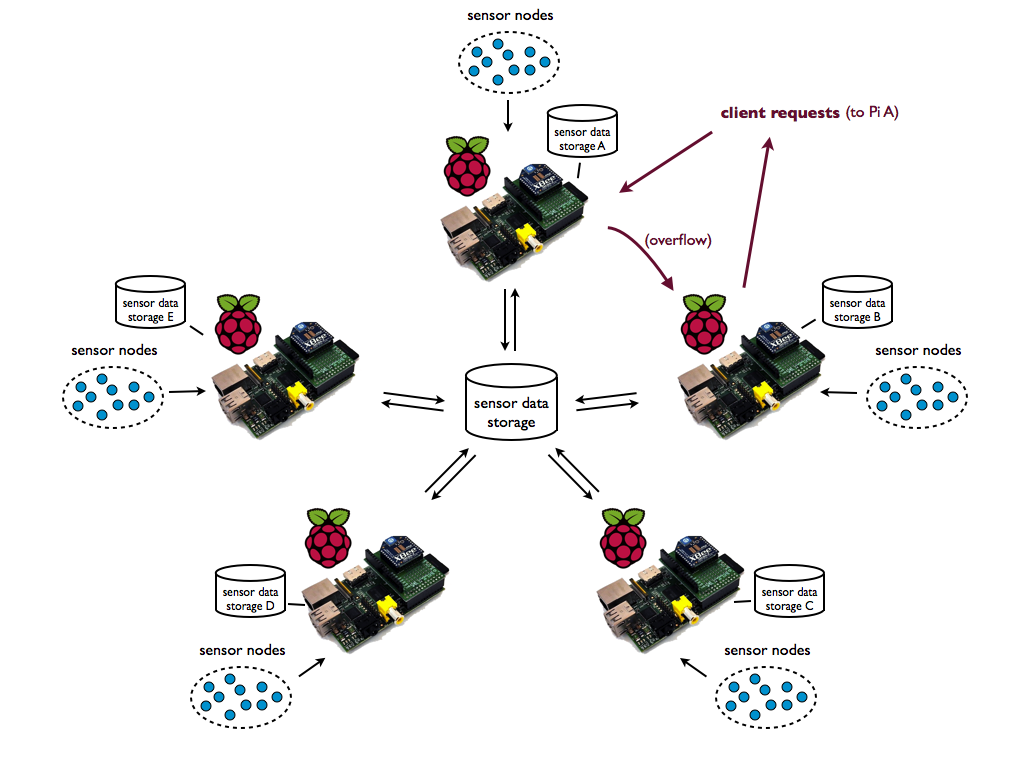
\includegraphics[width=0.5\textwidth]{architecture.png}
  \caption{\label{fig:parallel}Parallel form of the system architecture.}
\end{figure}

In a real-world scenario we would expect that user demands would gradually increase, with more sensors and more clients.  With this in mind we experimented with easy expansion of our system.  Our approach was a simple load-balanced division of sensors and clients, with a broadcast announcement when new devices are added, as illustrated in Figure~\ref{fig:parallel}.

Our example implementation involved two additional Raspberry Pi boards and facilities for them to communicate and load balance using Amazon Cloud Services as an intermediary data storage location.  This system is scalable and self-balancing.  Report to the central storage is done via the free tier of the Amazon EC2 (Elastic Compute Cloud) service that provides flexible and scalable capacity in the cloud.  Inter-Pi communication occurs using http requests over web sockets, as an addition to the current server infrastructure.

\begin{figure*}
  \centering
      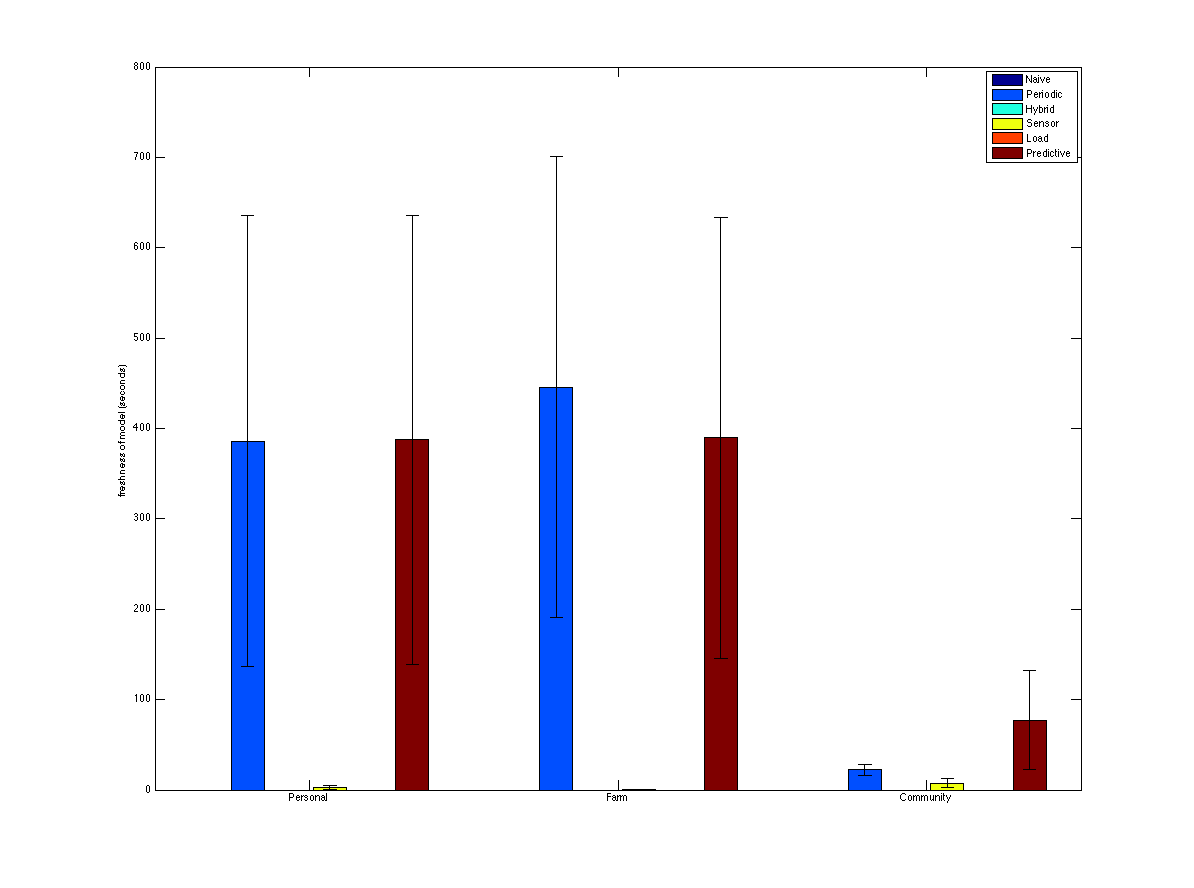
\includegraphics[width=0.48\linewidth]{freshness.png}
      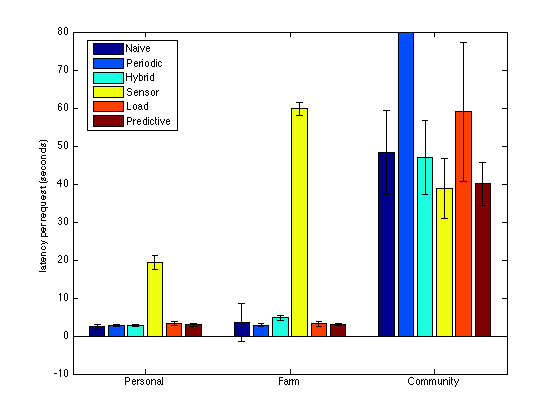
\includegraphics[width=0.48\linewidth]{latency_for_schedulers.png}
  \caption{\label{fig:main-results}Freshness (left) and latency (right) measurements for the six schedulers under three load types: personal, single user and five sensors, farm, single user and one hundred sensors, and community, fifty clients and one hundred sensors.}
\end{figure*}

\section{Evaluation}

It was not feasible to set up multiple sensors and run a live test over weeks, so we implemented a simulation harness to emulate the sensors and clients.  We ran all simulations with the server on the Raspberry Pi, and the mock sensors and clients on our own laptops. 

The harness was written in Python, using Tornado to manage queries.  We experimented with two methods of simulating clients, first with splinter \cite{} running actual firefox instances, to maximise realism, then with phantomjs \cite{}, which made large scale simulations much easier.  It was necessary to use a system capable of running JavaScript as the client's page is only considered to be "loaded" when the 15 most recent historical data points (transmitted via WebSockets, as described earlier) are delivered via JavaScript.

Client processes are forked from the main process: each client has a configurable list of plants from which list one plant is chosen randomly to query at each time step.  

\section{Results}

We simulated three scenarios for FRAICHE: personal garden, community garden, and small farm.  Each of these scenarios has a distinctive balance between clients and plants.  All simulations were performed on the Raspberry Pi with client requests and sensor updates issued from a MacBook Pro.

Client request batches were issued in 15 second time steps.  The number of clients making fresh requests was set to follow a sinusoidal pattern with some added noise.  Sensor update batches were also issued in 15 second time steps.  All sensors reported new data in every time period, though the updates were randomly spread across the period, to model the fact that the sensors would all be reporting periodically, but not be in sync.

Figure~\ref{fig:main-results} shows average results for measurements over fifteen minutes for each condition.  Freshness was tracked server side by the scheduler and logged every time a request is made.  Latency was measured on the client side and logged for each request.

\subsection{Personal Garden}

A personal garden is characterized by a single person caring for a small number of plants.  For the purposes of our simulation, we chose 5 to be a small number of plants: this scenario has one client and five plants.

\subsection{Community Garden}

PhantomJS

A community garden is made up of many people tending many plants.  We simulated 50 clients and 100 plants.

\subsection{Small Farm}

A small farm comprises many plants and a single farmer.  For our simulation, we ran one client and 100 plants.

\subsection{Client-side Modeling}

To evaluate the effectiveness of pushing the prediction modeling to the client browser, we ran an experiment that simulated a personal garden of five plants using the naive scheduler.  Using this approach, the average latency was X. We found this result (...)

\subsection{Load Balancing Between Pis}

Finally, we evaluated how the load balancing mechanism performed between multiple web servers. To simplify the scenario, we ran the experiment with two Raspberry Pis. We simulated a heavy loaded community garden condition with 50 clients requesting information to one RPi of 100 plants. This web server would redirect the overflow client request to another RPi that has low workload. We examined if the latency decreases after the targeted web server started forwarding the requests.

Figure~\ref{fig:parallel_result} shows the result of our experiment. (...)

\begin{figure}
  \centering
      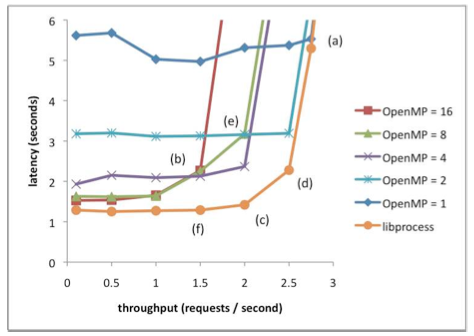
\includegraphics[width=0.5\textwidth]{multiplePis.png}
  \caption{\label{fig:parallel_result}Client request latency with load balancing between two web servers. [THIS FIGURE IS A PLACE HOLDER]}
\end{figure}

\section{Conclusions and Future Work}

In the future, we think it would be valuable to explore the space of very small commodity computers further.  There are many open questions relating to their performance for tasks

acquiring real-time weather conditions (e.g. weather.com XML format)

trigger on sensors

compare with other watering systems (ETO)

\section{REFERENCES}

1.	Barham, P., Dragovic, B., Fraser, K., et al. Xen and the art of virtualization. ACM SIGOPS Operating Systems Review 37, 5 (2003), 164-177.\\
2.	Cardell-Oliver, R., Smettem, K., and Kranz, M. Field testing a wireless sensor network for reactive environmental monitoring. International Conference on Intelligent Sensors, Sensor Networks and Information Processing, (2004).\\
3.	Ferguson, A.D., Bodik, P., Kandula, S., and Boutin, E. Jockey: Guaranteed Job Latency in Data Parallel Clusters. (2012).\\
4.	Ghodsi, A., Zaharia, M., Hindman, B., and Konwinski, A. Dominant resource fairness: fair allocation of multiple resource types. the USENIX Symposium on Networked Systems Design and Implementation (NSDI), (2011).\\
5.	Harchol-Balter, M. and Downey, A.B. Exploiting process lifetime distributions for dynamic load balancing. ACM Transactions on Computer Systems 15, 3 (1997), 253-285.\\
6.	Harish, V.C. and Owens, B. Dynamic Load Balancing DNS. Linux Journal 1999, 64es (1999).\\
7.	Lai, T.-T.T., Chen, Y.-H.T., Huang, P., and Chu, H.-H. PipeProbe. ACM Press (2010), 113-126.\\
8.	Litzkow, M.J., Livny, M., and Mutka, M.W. Condor-a hunter of idle workstations. the 8th International Conference on Distributed Computing Systems, (1988).\\
9.	Nichols, D. Using idle workstations in a shared computing environment. ACM SIGOPS Operating Systems Review, (1987).\\
10.	Pan, H., Hindman, B., and Asanović, K. Composing Parallel Software Efficiently with Lithe. ACM Sigplan Notices, (2010).\\
11.	Rowstron, A. and Druschel, P. Pastry: Scalable, Decentralized Object Location, and Routing for Large-Scale Peer-to-Peer Systems. In Middleware 2001. Middleware '01: the IFIP/ACM International Conference on Distributed Systems Platforms Heidelberg, Berlin, Heidelberg, 2001, 329-350.\\
12.	Stoica, I., Morris, R., Karger, D., et al. Chord: A scalable peer-to-peer lookup service for internet applications. ACM SIGCOMM Computer Communication Review 31, 4 (2001), 149-160.
13.	Tolle, G., Polastre, J., Szewczyk, R., and Culler, D. A macroscope in the redwoods. (2005).\\
14.	Waldspurger, C.A. and Weihl, W.E. Lottery Scheduling: Flexible Proportional-Share Resource Management. (1994).

\bibliography{bib}
\bibliographystyle{plainnat}
\end{document}
